\section{Resultados} % ESSA É CRITÈRIO AVALIATIVO
%Tòpicos avalistivos: 3 e 4
% SINTO MUITO, FICOU GIGANTE. FIQUEM À VONTADE PARA ALTERAR EU TENTEI POR SÓ O ESSENCIAL. Acho que vão concordar que fui bastante sucinto para o tanto de resultado e a clareza da apresentação.

Como a deriva decorre em um processo estocástico, é importante examinar o que acontece em várias corridas diferentes de simulação para obter uma visão mais global do processo. Para tanto, nossa primeira visualização foi acompanhar o que acontece com o tamanho do genoma (aqui aproximado pelo tamanho médio do genótipo) de uma população de mesmo tamanho em 15 simulações com mesmos parâmetros, mas números aleatórios diferentes. Este resultado está resumido na \cref{fig_runs} para duas populações diferentes, uma com 100 e outra com 1000 indivíduos.

\begin{minipage}{\linewidth}
    (A) 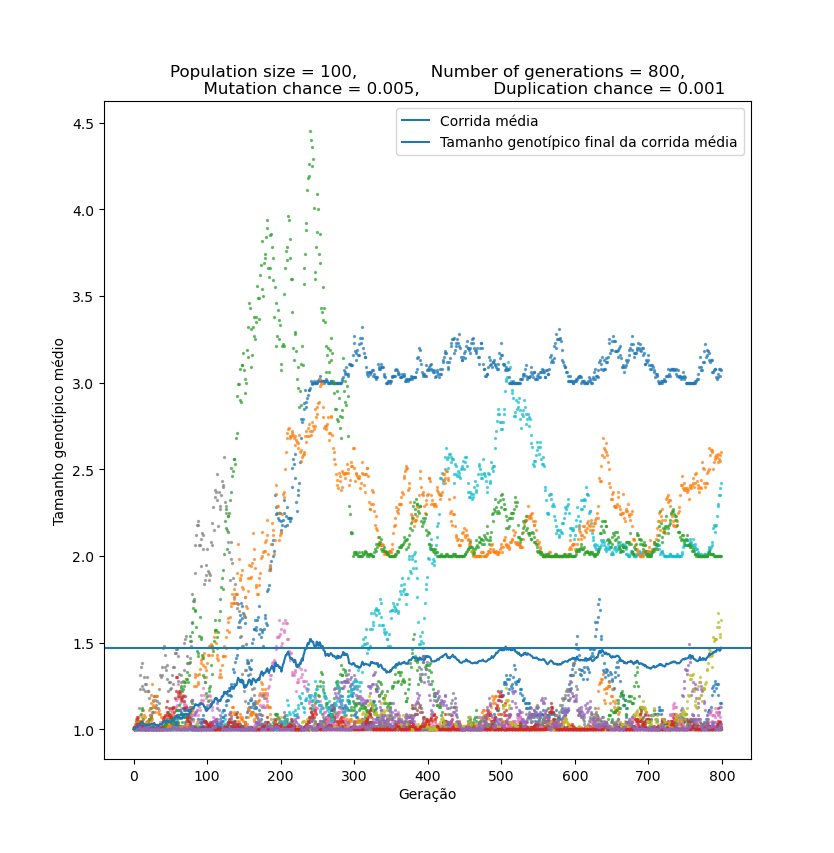
\includegraphics[width=.45\linewidth]{figs/5_100individuals_geneCloneCost.png}
    (B) 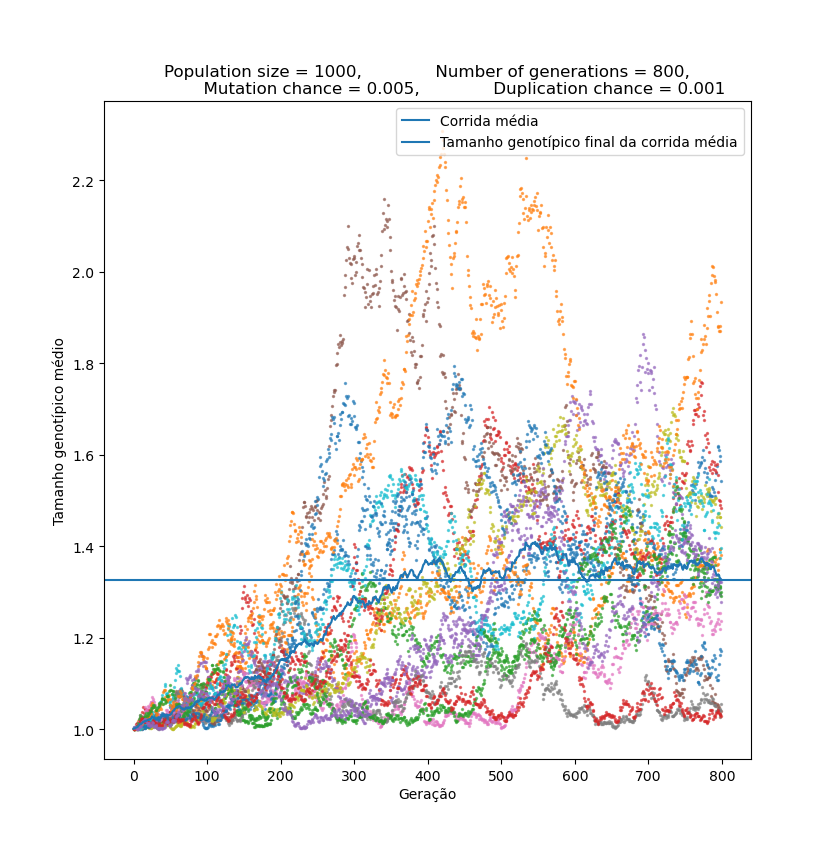
\includegraphics[width=.45\linewidth]{figs/5_1000individuals_geneCloneCost.png}
        \captionof{figure}{Gráficos gerados após 15 simulações de duas populações, uma com 100 indivíduos (A) e outra com 1000 indivíduos (B). Em pontilhado estão resultados de cada corrida medindo o tamanho médio do genótipo dos indivíduos da população em função do tempo (número de gerações). A linha contínua é a "corrida média", isto é, a média do tamanho médio do genótipo a cada geração. A linha horizontal por sua vez marca a média do tamanho médio final do genótipo}\label{fig_runs}
\end{minipage}
\vspace{1em}

É notável que as escalas dos gráficos resultantes são diferentes. Para 100 indivíduos o tamanho máximo do genoma é quase o dobro do caso de 1000 indivíduos. Embora pouco convincente estatisticamente, este resultado inicial ilustra o argumento de Lynch e ataca uma das principais críticas.

Para melhor observar o fenômeno, prosseguimos com uma avaliação mais sistemática do que acontece com o tamanho do genoma ao variar o tamanho da população. Para isso, escolhemos observar o que acontece na média de 15 simulações para cada tamanho de população variando de 10 indivíduos até 1010 indivíduos de 100 em 100. Ou seja, simulamos o que está demonstrado na \cref{fig_runs} para cada tamanho de população de 10 até 1010 indivíduos com passo de 100 indivíduos entre uma população e outra. Os resultados estão ilustrados na \cref{fig_graphs} (A). 

No entanto, é preciso entender qual viés é gerado por cada variável. Isto é, avaliar como, para um dado tamanho populacional, a chance de mutação e o custo por gene no genótipo variam o tamanho médio do genoma. Assim, uma simulação similar à da variação do tamanho populacional foi proposta para cada uma dessas variáveis, variando a chance de mutação conforme descrito na \cref{fig_graphs} (B) e o custo por gene no genótipo conforme descrito na \cref{fig_graphs} (C).

\begin{minipage}{\linewidth}
    \centering
    (A) 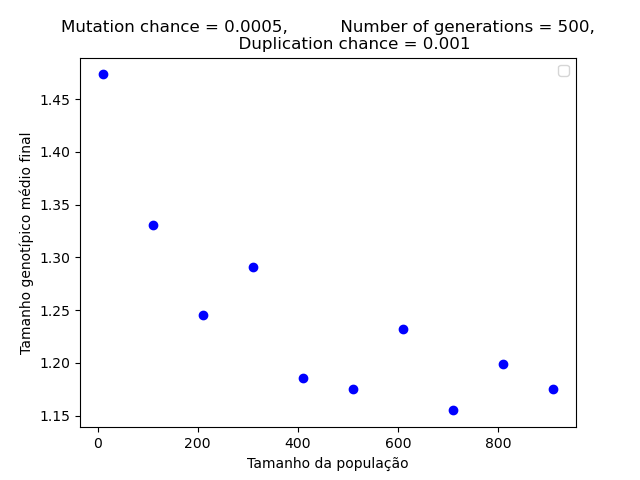
\includegraphics[width=.65\linewidth]{figs/population_variation.png}
    \\(B) 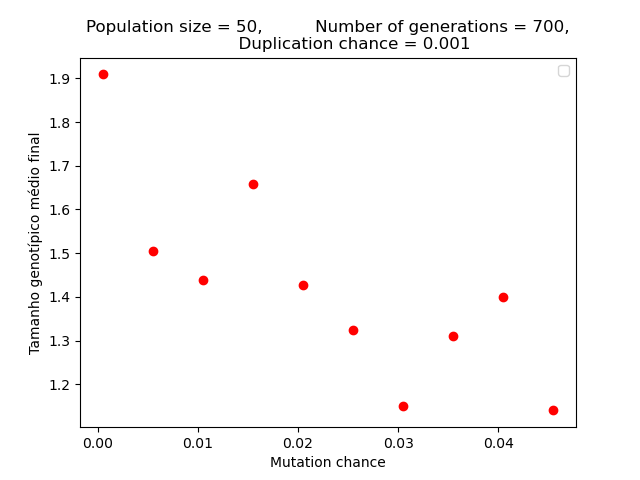
\includegraphics[width=.45\linewidth]{figs/mutation_variation.png}
    (C) 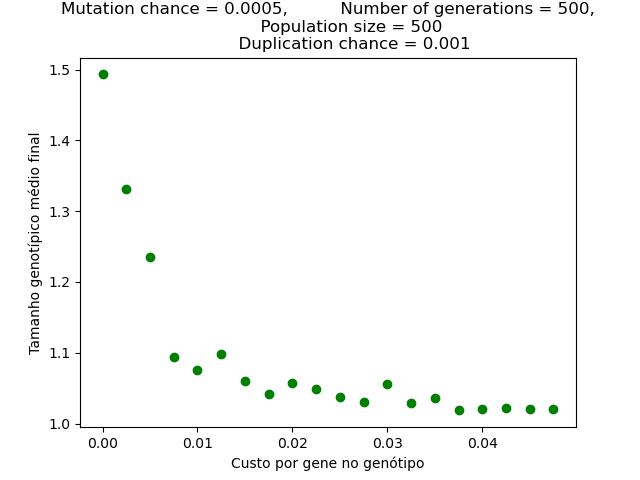
\includegraphics[width=.45\linewidth]{figs/gene_cost_variation.png}
    \captionof{figure}{Gráficos gerados através da média de 15 simulações para cada parâmetro. Em (A) o tamanho da população varia de 10 até 1010 com passo de 100 indivíduos. Em (B) a chance de mutação varia de 0.0005  até 0.05 com passo de 0.005 entre uma população e outra. Em (C) o custo por gene extra variou de 0 à 0.05 com passo de 0.0025 entre uma população e outra.}\label{fig_graphs}
\end{minipage}
\vspace{1em}

A variação do tamanho médio do genótipo com a chance de mutação e o custo por gene evidenciam o bom comportamento do código. Como as mutações disponíveis eram deletérias em uma proporção de 50:1 com relação a mutações neutras e nenhuma vantajosa, o esperado era de fato que o tamanho do genótipo decaísse com o aumento na chance de um gene mutar para uma versão deletéria. Similarmente, remover o custo por simplesmente ter um gene a mais aumenta drasticamente o tamanho do genoma final em comparação a um custo ainda pequeno de 0.01. Assim, os resultados obtidos são coerentes com as premissas.

A diminuição do tamanho do genoma final em populações maiores indica a troca de um ambiente mais propenso à deriva genética aleatória para um dominado pela seleção, mantendo o valor médio final cada vez mais próximo de 1. Este achado é coerente com o proposto por Lynch e Conery, ilustrando a importância da população geneticamente disponível para a possibilidade de aumentar um genótipo apenas através de acúmulo de genes ``inúteis''. É importante observar algo muito bem ilustrado na \cref{fig_runs} (A), nem toda população menor apresenta genótipos maiores, o efeito de deriva permite o acúmulo de genótipos maiores, mas não garante que ocorra. Similarmente, em populações maiores genótipos maiores podem surgir, mas a tendência é que a força da seleção os remova.


\subsection{Comparação com trabalhos anteriores} %ESSA É CRITÉRIO DE AVALIAÇÃO
%Tópico avaliativo 2 e 4

COMPARAR COM TRABALHOS ANTERIORES E TALS


